\documentclass[12pt]{article}
\usepackage[margin=2.5cm]{geometry}
\usepackage{enumerate}
\usepackage{amsfonts}
\usepackage{amsmath}
\usepackage{fancyhdr}
\usepackage{amsmath}
\usepackage{amssymb}
\usepackage{amsthm}
\usepackage{mdframed}
\usepackage{graphicx}
\usepackage{subcaption}
\usepackage{adjustbox}
\usepackage{listings}
\usepackage{xcolor}
\usepackage{booktabs}
\usepackage[utf]{kotex}
\usepackage{hyperref}

\definecolor{codegreen}{rgb}{0,0.6,0}
\definecolor{codegray}{rgb}{0.5,0.5,0.5}
\definecolor{codepurple}{rgb}{0.58,0,0.82}
\definecolor{backcolour}{rgb}{0.95,0.95,0.92}

\lstdefinestyle{mystyle}{
    backgroundcolor=\color{backcolour},
    commentstyle=\color{codegreen},
    keywordstyle=\color{magenta},
    numberstyle=\tiny\color{codegray},
    stringstyle=\color{codepurple},
    basicstyle=\ttfamily\footnotesize,
    breakatwhitespace=false,
    breaklines=true,
    captionpos=b,
    keepspaces=true,
    numbers=left,
    numbersep=5pt,
    showspaces=false,
    showstringspaces=false,
    showtabs=false,
    tabsize=1
}

\lstset{style=mystyle}

\pagestyle{fancy}
\renewcommand{\headrulewidth}{0.4pt}
\lhead{Team Treehouse}
\rhead{Modifying Data with SQL Part 2 Notes}

\begin{document}
\title{Modifying Data with SQL Part 2 Notes}
\author{Team Treehouse}
\maketitle

\bigskip

\section{Updating All Rows in a Table}

\bigskip

\begin{itemize}
    \item \textbf{Syntax:} UDPATE \textit{table name} SET \textit{column 1 name} = \textit{value 1 name}, \textit{column 2 name} = \textit{value 2 name};

    \begin{lstlisting}[language=SQL]
    UPDATE users SET password = "thisisabadidea";


    UPDATE products SET price = 2.99;


    UPDATE users SET first_name = "Anony", last_name = "Moose";


    UPDATE products SET stock_count = 0, price = 0;
    \end{lstlisting}
\end{itemize}


\bigskip

\section{Updating Specific Rows}

\bigskip

\begin{itemize}
    \item \textbf{Syntax:} UPDATE \textit{table name} SET \textit{column 1 name} = \textit{value 1 name}, \textit{column 2 name} = \textit{value 2 name} WHERE \textit{condition};

    \begin{lstlisting}[language=SQL]
    UPDATE users SET password = "thisisabadidea" WHERE id = 3;


    UPDATE blog_posts SET view_count = 1923 WHERE title = "SQL is Awesome";


    UPDATE users SET entry_url = "/home", last_login = "2016-01-05" WHERE id = 329;


    UPDATE products SET status = "SOLD OUT", availability = "In 1 Week" WHERE stock_count = 0;
    \end{lstlisting}
\end{itemize}

\bigskip

\section{Exercise 1}

\bigskip

\begin{itemize}
    \item Solution included in \textit{exercise\_1.sql}
\end{itemize}

\bigskip

\section{Review and Practice}


\bigskip

\section{Quiz 1}

\bigskip

\begin{enumerate}[1.]
    \item

    Please fill in the correct answer in each blank provided below.

    \bigskip

    Fill in the missing keywords for the following UPDATE statement.

    \bigskip

    \begin{lstlisting}[language=SQL]
    UPDATE users SET password = "thisisabadidea" WHERE id = 3;


    UPDATE blog_posts SET view_count = 1923 WHERE title = "SQL is Awesome";


    UPDATE users SET entry_url = "/home", last_login = "2016-01-05" WHERE id = 329;


    UPDATE products SET status = "SOLD OUT", availability = "In 1 Week" WHERE stock_count = 0;
    \end{lstlisting}


    \item

    \begin{center}
    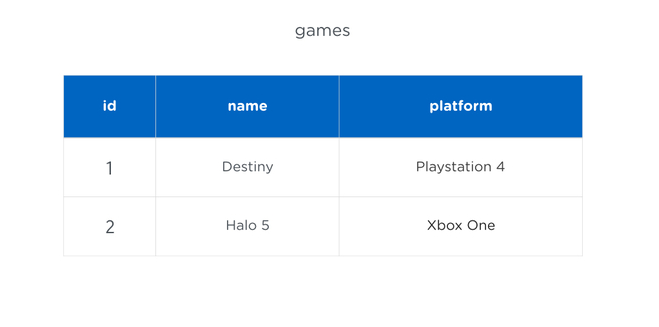
\includegraphics[width=0.8 \linewidth]{images/part_2_notes_1.png}
    \end{center}

    After issuing the following statement, what would you expect the contents of the table to be?

    \bigskip

    \begin{lstlisting}[language=SQL]
    UPDATE games SET platform="Cross-Platform";
    \end{lstlisting}

    \bigskip

    \begin{enumerate}[A.]
        \item

        \begin{tabular}{|c|c|c|}
        \hline
        id  &	name    &	platform\\
        \hline
        1   &	Destiny &	Playstation 4\\
        \hline
        2   &	Halo 5  &	Xbox One\\
        \hline
        \end{tabular}

        \item

        \begin{tabular}{|c|c|c|}
        \hline
        id  &	name    &   platform\\
        \hline
        1   & 	Destiny &	Cross-Platform\\
        \hline
        2   &	Halo 5  &	Xbox One\\
        \hline
        \end{tabular}

        \item

        \begin{tabular}{|c|c|c|}
        \hline
        id  &	name    &	platform\\
        \hline
        1   &	Destiny &	Cross-Platform\\
        \hline
        2   &	Halo 5  &	Cross-Platform\\
        \hline
        \end{tabular}

    \end{enumerate}

    \bigskip

    \textbf{Answer:} C

    \item

    \begin{center}
    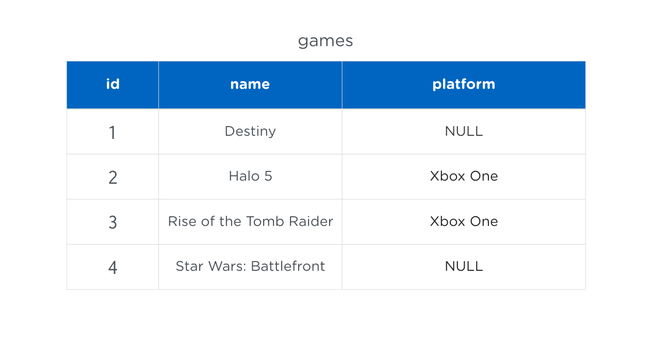
\includegraphics[width=0.8 \linewidth]{images/part_2_notes_2.png}
    \end{center}

    \bigskip

    Please fill in the correct answer in each blank provided below.

    \bigskip

    Finish the following statement to replace NULL values with the value of "Cross-Platform".

    \bigskip

    \begin{lstlisting}[language=SQL]
    UPDATE games SET platform = "Cross-Plaform" WHERE id \_\_\_ (1,4);
    \end{lstlisting}

    \bigskip

    What is the missing operator?

    \bigskip

    \textbf{Answer:} IN


    \item

    Please fill in the correct answer in each blank provided below.

    \bigskip

    Fill in the missing keywords for the following UPDATE statement.

    \bigskip

    \begin{lstlisting}[language=SQL]
    UPDATE shows SET title \_\_\_  "Friends";
    \end{lstlisting}

    \bigskip

    What is the missing operator?

    \bigskip

    \textbf{Answer:} =


\end{enumerate}

\end{document}